\documentclass[a4paper]{scrartcl}
\usepackage{mathe-blatt}
\usepackage{graphicx}
\usepackage{listings}
\blattnumeins

\begin{document}

\begin{aufgabe}
	\begin{enumerate}[a)]
		\item
			Sei $A$ regulär, dann erfüllt $A^{-1}$ die Penrose-Bedingungen:
			\begin{enumerate}[i)]
				\item
					$AA^{-1}A = A$
				\item
					Folgt aus i) und der Kommutativität von $A$ und $A^{-1}$.
				\item
					$(AA^{-1})^* = I^* = I = AA^{-1}$
				\item
					Folgt aus iii) und der Kommutativität von $A$ und $A^{-1}$.
			\end{enumerate}
			Also ist $A^{-1} = A^+$.
		\item
			Folgt direkt aus der Vertauschbarkeit von $A$ und $B:=(A^+)^+$ in den Penrose-Bedingungen.
		\item
			Zeige: $(A^+)^*$ erfült die Penrosebedingungen für die Matrix $A^*$:
			\begin{enumerate}[i)]
				\item
					$A^*(A^+)^*A^* = (AA^+A)^* = A^*$
				\item
					$(A^+)^*A^*(A^+)^* = (A^+AA^+)^* = (A^+)^*$
				\item
					$(A^*(A^+)^*)^* = A^+A = (A^+A)^* = A^*(A^+)^*$
				\item
					$((A^+)^*A^*)^* = AA^+ = (AA^+)^* = (A^+)^*A^*$
			\end{enumerate}
		\item
			Das ist mir nicht ersichtlich.
			Verwende b), e) und die Regel $A^+ = A^*(AA^*)^+$, welche sich analog zu e) zeigen lässt:
			\begin{align*}
				&(AA^+)^+ 
				= \Big((AA^+)^*(AA^+)\Big)^+(AA^+)^*
				= (AA^+)AA^+\\
				&\quad= (AA^+)^*\Big((AA^+)(AA^+)^*\Big)^+ AA^+
				= AA^+(AA^+)^+AA^+ \\
				&\quad= AA^+
				= (A^+)^+A^+
			\end{align*}
			womit Gleichheit gelten sollte.
			Allerdings gilt im Allgemeinen \emph{nicht} $(AB)^+ = B^+A^+$.
		\item
			Zeige zunächst $(A^*A)^+ = A^+(A^*)^+$ anhand der Penrose-Bedingungen:
			\begin{enumerate}[i)]
				\item
					$A^*AA^+(A^*)^+A^*A = A^*AA^+AA^+A = A^*A$
				\item
					$A^*(A^*)^+A^*AA^+(A^*)^+ = A^+AA^+AA^+(A^*)^+ = A^+(A^*)^+$
				\item
					$\big(A^*AA^*(A^*)^+\big)^* = A^+AA^+A = (A^+AA^+A)^* = A^*AA^+(A^*)^+$
				\item
					$\big(A^+(A^*)^+A^*A\big)^* = (A^+AA^+A)^* = A^+AA^+A = A^+(A^*)^+A^*A$
			\end{enumerate}
			Dann gilt einfach:
			\[
				A^+ = A^+AA^+ = A^+(AA^+)^* = A^+(A^*)^+A^* = (A^*A)^+A^*
			\]
		\item
			Da $A$ vollen Spaltenrang hat, ist die Grammatrix $A^*A$ invertierbar.
			Der Rest folgt aus e).
	\end{enumerate}
\end{aufgabe}
\newpage
\begin{aufgabe}
	\begin{enumerate}[a)]
		\item
			Zeige, dass jedes $z\in V$ auf sich selber abgebildet wird.
			$P\cdot 0 = 0$ ist offensichtlich, da $P$ linear.
			Sei $0\neq z \in V$, dann gilt wegen der positiven Definitheit des Skalarprodukts
			\[
				\<z-Pz,z\> = 0 \implies z-Pz = 0 \implies Pz=z
			\]
			und damit $P=P^2$.
		\item
			Sei $z\in V^\orth$ und $y\in \C^m$
			\[
				\<y-(I-P)y,z\> = \<Py,z\> = 0
			\]
			da $Py \in V$.
			Damit ist $\Id - P$ eine orthogonale Projektion auf $V^\orth$.
		\item
			Nutze $Py\in V$ und die Eigenschaft der Projektion:
			\begin{align*}
				\|y-z\|^2
				&=\<y-Py,y-Py\> + \<Py-z,Py-z\> \\
				&= \<y,y\> - \<y,Py\> - \<Py,y\> + \<Py,Py\> + \<Py,Py\> - \<Py,z\> - \<z,Py\> + \<z,z\>\\
				&= \<y,y\> + \underbrace{\<Py-y,Py\>}_{=0} + \underbrace{\<Py,Py-y\>}_{=0} -\<y,z\> + \<y,z\> - \<Py,z\> - \<z,y\>+\<z,y\> - \<z,Py\> + \<z,z\>\\
				&= \<y,y\> - \<y,z\> + \underbrace{\<y-Py,z\>}_{=0} - \<z,y\> + \underbrace{\<z,y-Py\>}_{=0} + \<z,z\> \\
				&= \<y-z,y-z\> = \|y-z\|^2
			\end{align*}
		\item
			Nach c) gilt
			\[
				\min_{z\in V} \|y-z\|^2 = \|y-Py\|^2 + \underbrace{\min_{z\in V}\|Py-z\|^2}_{=0 \text{ für $z=Py\in V$}} = \|y-Py\|^2
			\]
	\end{enumerate}
\end{aufgabe}

\begin{aufgabe}
	\begin{enumerate}[a)]
		\item
			Die Fehlerberechnung:
			\lstinputlisting[language=matlab]{num1_6_4/error.m}
			Die Visualisierung:
			\lstinputlisting[language=matlab]{num1_6_4/a.m}
			\begin{figure}[h]
				\centering
				\caption{Der relative Approximationfehler in Abhängigkeit von $k$}
				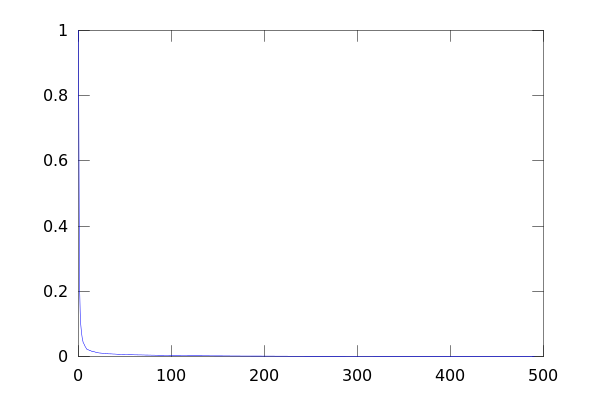
\includegraphics[scale=0.6]{num1_6_4/error.png}
			\end{figure}
\newpage
		\item			
			Der Quellcode:
			\lstinputlisting[language=matlab]{num1_6_4/b.m}
			\begin{table}[h]
				\centering
				\caption{Mindestrang für Approximation mit gegebenem Fehler und Anzahl zu Speichernder Koeffizienten bei der SVD}
				\begin{tabular}{c|r|r}
					Fehler & $k$ & Koeffizienten für die verkürzte SVD \\ \hline
					10\% & 3 & 4083 \\
					5\% & 5 & 6805 \\
					1\% & 26 & 35386 \\
					0.1\% & 211 & 287171 
				\end{tabular}
			\end{table}

			\begin{figure}[h]
				\centering
				\caption{Die Ausgaben der Approximationen für $k\in \{3,5,26,211\} $ }
				\begin{tabular}{c}
					
\includegraphics[scale=0.4]{num1_6_4/k3.png} 
					\\ 
\includegraphics[scale=0.4]{num1_6_4/k5.png} \\
					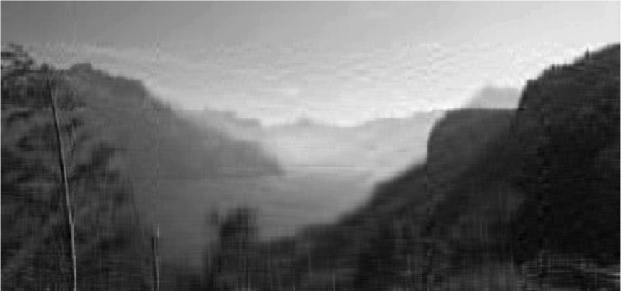
\includegraphics[scale=0.4]{num1_6_4/k26.png} 
					\\ 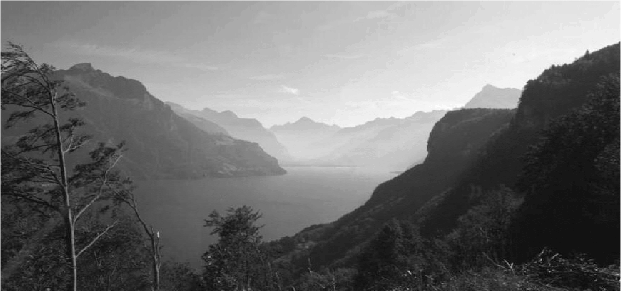
\includegraphics[scale=0.4]{num1_6_4/k211.png}
				\end{tabular}
			\end{figure}
	\end{enumerate}
\end{aufgabe}

\end{document}
